\subsubsection*{Initialize plant parameters from scratch} 
 
In the previous examples we opened the plant parameters from an XML file. In the following example we demonstrate how to construct a plant with a Python script without the need of any parameter file. This is especially important, if we want to modify parameters in our scripts (e.g. like it is needed for a sensitivity analysis, see Section \ref{ssec:sa}). \\

In order to set up a simulation by hand, we have to define all relevant model parameters. This is done by creating a RootRandomParameter, a StemRandomParameter, and a LeafRandomParameter object for each organ order or organ sub-type, and a single SeedRandomParameter for each plant type. In this section we will show how to create parameter sets, modify parameters and write XML plant parameter files. In Section \ref{sec:cplantobx} we present a detailed model description including all organ parameters. \\

Note that during the simulation, the parameters for a specific organ (i.e. OrganSpecificParamter with the specialisations RootSpecificParameter, StemSpecificParameter, and LeafSpecificParameter) are generated from the OrganRandomParameter class (with the specialisations RootRandomParameter, StemRandomParameter, and LeafRandomParameter ) which represents the random distributions of certain parameters. First, we show how to construct instances of these classes, and show their parameters. \\


\lstinputlisting[language=Python, caption= How to create random parameter sets (specialisations of OrganRandomParameter) (topics\_parameters2.py)]{examples/topics_parameters.py}


\lstinputlisting[language=Python, caption= A root system from scratch (topics\_parameters2.py)]{examples/topics_parameters2.py}

\begin{itemize}
\item[5] Matplotlib is Python's easy way to create figures like in Matlab.\item[6] NumPy is Python's scientific computing package.
\item[9,10] Create the root type parameters of type 1 and type 2.
\item[12-38] We set up a simple root system by hand. First we define the tap root L12-L26, then the laterals L28-L38. By default all standard deviations are 0. Most parameters standard deviations can be set with an additional 's' appended to the parameter name, e.g. $lmaxs$ is the standard deviation of $lmax$, see L32
\item[40,41] Set the root type parameters.
\item[43-47] Create an object of class SeedRandomParameter which defines when basal and shoot borne roots emerge. In this example we neglect basal and shoot borne roots, and just define the seed location, and deactivate basal roots by setting their maximal number $maxB$ to 0 ($firstB$ and $delayB$ are ignored in that case). 
\item[48] Sets the root system parameters.
\item[53] We choose the simulation times in a way that we can see the temporal development, and that all lateral roots have emerged in the final time step.
\item[54-70] Within the simulation loop we create Figure \ref{fig:ip}. L58-61 defines the limits and titles. In L63 we retrieve the roots as polylines which are represented by a list of nodes. In L64-67 we plot the $x$ and $z$ coordinates for each segment ($n$, $n2$) as green line. 
\item[75-80] It is not only possible to set all model parameter, 
but to retrieve the parameters after the simulation with rs.getParameter(), which returns one value per root. For all parameters that are derived from a random distribution the root specific parameter is returned (e.g. $la$, L78), i.e. the values that were drawn from the normal distribution. The root random parameter can be accessed by adding '\_mean', '\_dev' to the parameter value (e.g. $la\_mean$, L79).
\end{itemize}

Note that all parameters can be set and modified within Python. Especially, standard deviations can be set to zero in order to be able to precisely predict the result. For example we can calculate the total root system length analytically, and check if the numerical simulation yield the (exact) same result. This is performed in the tests test\_root.py, and test\_rootsystem, which is used to test and validate CPlantBox (see folder CPlantBox/test).

With such simple simulations, we can quickly check if the model does, what we expect. For example the maximal number of laterals of above parameters is 16 
$= round(lmax - la - lb)/l_n +  1$. We can calculate the time when the final lateral emerges as $-(lmax/r)*\ln(1-(lmax-l_n/2)/lmax)$ = 122.8 days. At simulation time 125 the last lateral root that has emerged is 2.2 days old, and therefore approximately 4.4 cm long (initial growth rate $r_1 = 2$), which agrees with Figure \ref{fig:ip}.

By default the length of the apical zone is fixed, when the root is created. During growth the apical zone stays in the interval $[la - l_n/2, la+l_n/2]$. The first branch emerges at length $lb$, when the root length reaches $lb +la$.

In the following two subsections we show, how tropism parameters and inter lateral spacing will affect the resulting root system.

% \begin{figure}
% \centering
% \includegraphics[width=\textwidth]{figures/topics_parameters2.png}
% \caption{Root development} \label{fig:ip}
% \end{figure}

\subsubsection*{Modify inter-lateral spacing (ln, lnk)} 

A single root is divided in basal zone, root branching zone, and root apical zone. Basal and apical zone are given by the parameters $la$, and $lb$ with standard deviations $la_s$ and $lb_s$. The branching zone has the size $lmax-la-lb$, where $lmax$ is the maximal root length. The branching zone is divided into inter lateral distances $l_n$, which are values drawn from a normal distribution with standard deviation $l_{ns}$. All values are fixed when the root is created This is performed in the method RootRandomParameter::realize(). The chosen parameters reflect the root growth under perfect conditions. Based on this, the root development can then be influenced by environmental conditions e.g. impeding growth speed, or lateral emergence, see Section \ref{sec:functional}.

Normally, the setting constant branching distances is sufficient, but sometime experimental data indicate that inter lateral distances are smaller, or larger near the base than near the root tip. The reason for this could be soil root interaction (e.g. root response to dense or nutritious layer), or within the genotype. We added a purely descriptive parameter to mimic such experimental observations. The parameter $lnk$, which is zero per default, defines the slope, at the mid of the branching, altering the inter lateral distance linearly along the root axis. In the following script, we demonstrate the usage of $lnk$.

\lstinputlisting[language=Python, caption=Example 2c (topics\_parameters2.py)]{examples/topics_parameters2.py}

\begin{itemize}
\item[10-13] A root system with a single tap root is created. 
\item[16,16] The axial resolution, and insertion angle is defined. We take a very large axial resolution for the tap root, since we visualize the nodes later on, and we want to see only lateral branching nodes.
\item[18-24] Definition of the tap root. Standard deviations are zero, we do not want any variations. Tropism parameters are chosen in a way, that the tap root grows straight downwards.
\item[26-29] Definition of the first order lateral. Tropism is a strict exotropism (i.e. root follows its initial growth direction).
\item[31,32] The parameter values we want to visualize.
\item[36] Resets the root system (to $simTime = 0$). Root parameters are not changed. 
\item[38,39] Sets the values for this subplot. 
\item[41,42] Runs the simulation
\item[44-56] Creates the subplots. First (L47-49) we plot all segments in green. And second (L51-53) we plot all nodes of the tap root as red asterisks.
\item[58-60] Creates Figure \ref{fig:spacing}
\end{itemize}

The mid column of Figure \ref{fig:spacing} shows to different inter lateral distances, 4 (top) and 2 (cm) bot. The left column demonstrate the use of negative values for $lnk$ which results in larger distances near the base. The right column has positive values for $lnk$, which will result in smaller distances near the base. The $i$-th inter distance is calculated as $ln_i = ln + lnk (x_i-mid_x)$, where $x_i$ is the position within the branching zone, and $mid_x$ is the mid of the branching zone. This is done in RootRandomParameter::realize(). Note that $lnk$ is dimensionless and the slope in the linear equation. At mid of the branching zone the inter-lateral distance equals $ln$. 

% \begin{figure}
% \centering
% 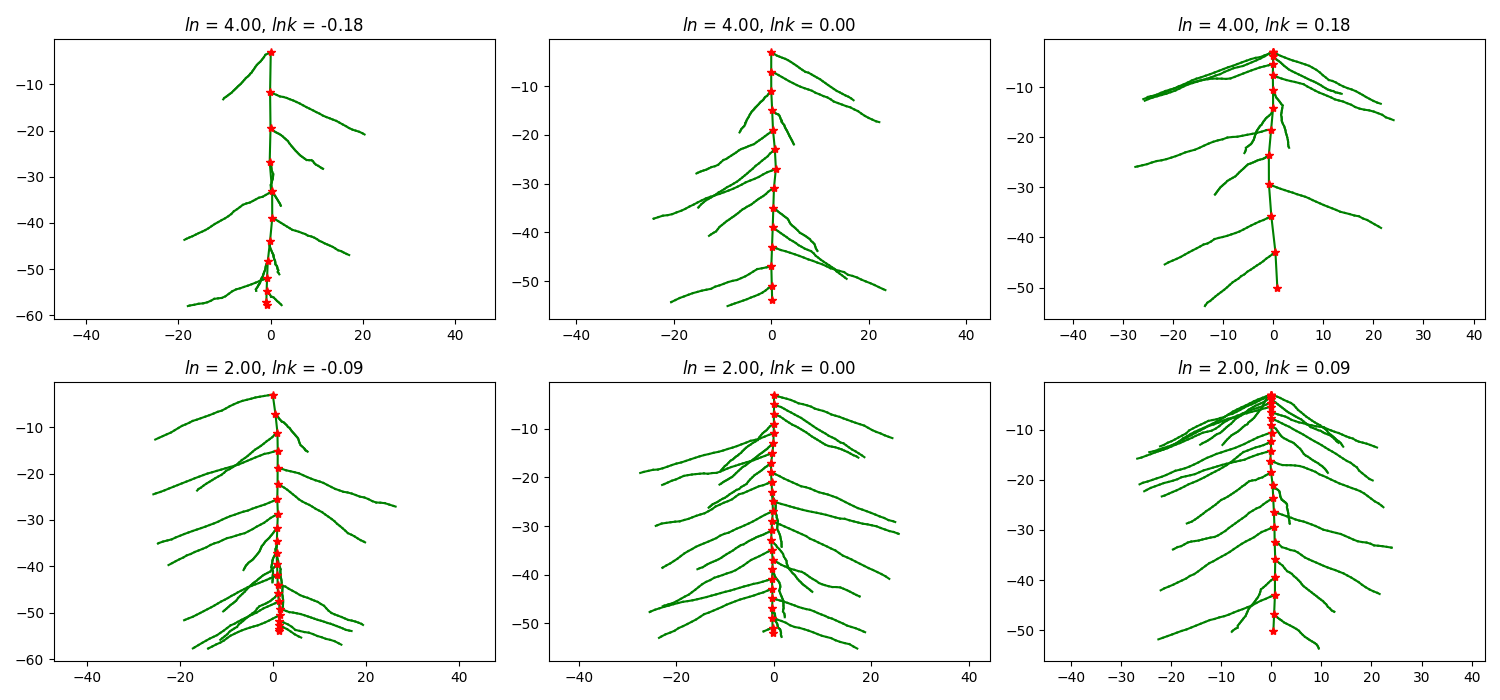
\includegraphics[width=0.99\textwidth]{fig_lateralspacing.png}
% \caption{Inter-lateral spacing, larger near base (left column), constant (mid column), and smaller near base (right column) } \label{fig:spacing}
% \end{figure}

In the following we show, how to analyse model results on a per root basis using the RootSystem class. To create density distributions the resulting root segments are analysed using the SegmentAnalyser class, described in Section \ref{sec:sa}.


\lstinputlisting[language=Python, caption=Example 2c (topics\_parameters3.py)]{examples/topics_parameters3.py}



